\documentclass{article}
\usepackage[utf8]{inputenc}
\usepackage{polski}
\usepackage[T1]{fontenc}
\usepackage{amsmath,amssymb,amsthm}
\usepackage{lmodern}
\usepackage{geometry}
\usepackage[dvipsnames]{xcolor}
\usepackage{hyperref}
\usepackage{array}
\usepackage{graphicx}
\usepackage{caption}

\newtheorem{tw}{Twierdzenie}[section]
\newtheorem{lem}{Lemat}[section]

\begin{document}

\begin{center}
    \LARGE
    \textbf{Pracownia z Analizy numerycznej (M)}

    \medskip

    Sprawozdanie do zadania {\bf P1.4}
    
    %{\Large Prowadzący: Filip Chudy}

    \bigskip

    {\Large Jadwiga Świerczyńska}
    
    {\Large Wrocław, 18.11.2022 r.}
    
\end{center}

\vspace{70pt}

\section{Wstęp}

Ciągi, czyli funkcje ze zbioru liczb naturalnych w pewien inny zbiór, są używane w niemal każdej nauce ścisłej, a w szczególności są podstawą analizy matematycznej. Wyznaczanie kolejnych wyrazów ciągu może mieć wieloraki cel - na przykład może posłużyć do przybliżania wartości granicy ciągu.

Wiele ciągów wyraża się skomplikowanym wzorem, przez to obliczanie ich wyrazów tradycyjnie tj. bez użycia komputera, może nastręczyć trudności. Badanie różnych sposobów jest zatem zadaniem nie tylko ważnym, ale także bardzo często spotykanym. Niestety metody używające komputera niosą ze sobą pewne ryzyko błędu numerycznego. W wielu przypadkach nie jest możliwe uzyskanie dokładnego wyniku, aczkolwiek programista może wpłynąć na wielkość odchylenia od prawdziwej wartości.

W poniższym sprawozdaniu porównano różne metody obliczania kolejnych wyrazów ciągu zadanego następującym wzorem jawnym:
\begin{equation}\tag{WJaw}
    \label{wzor_jaw}
    x_k = A(1+\sqrt{3})^k + B(1-\sqrt{3})^k \text{.}
\end{equation}

W badaniach użyto wzoru jawnego oraz rekurencyjnego, którego poprawność jest opisana w rozdziale \ref{rek}. Wyrazy ciągu obliczano przy pomocy programu napisanego w języku \verb|Julia| w arytmetykach \verb|single| (32 bity)  i \verb|double| (64 bity).

\newpage

\section{Zależność rekurencyjna}
\label{rek}
W tej sekcji udowodnimy, że zależność rekurencyjna, z której korzystamy, jest poprawna oraz wyliczymy stałe \(A, B\) dla ustalonych \(x_1, x_2\).

\begin{lem}
    \label{lem:rek}
    Dla dowolnych stałych \(A,B\) ciąg
    \[
        x_k = A(1+\sqrt{3})^k + B(1-\sqrt{3})^k
    \]
    spełnia związek rekurencyjny
    \begin{equation}\tag{WRek}\label{wzor_rek}
        x_k = 2(x_{k-1} + x_{k-2}) \quad\quad (k=3, 4, \ldots) \text{.}
    \end{equation}
        
\end{lem}

\begin{proof}
    Korzystając ze wzoru jawnego na ciąg \(x_k\), przeprowadzamy następujący rachunek.
    \begin{align*}
        % jak zrobić ładne align przy stackrelu?
        2(x_{k-1} + x_{k-2}) &\stackrel{\text{def.}}{=} 
        2\left(  A(1+\sqrt{3})^{k-1} + B(1-\sqrt{3})^{k-1} +  A(1+\sqrt{3})^{k-2} + B(1-\sqrt{3})^{k-2} \right) \\
        &= 2\left( A(1+\sqrt{3})^{k-2}(1+\sqrt{3}+1) + B(1-\sqrt{3})^{k-2}(1-\sqrt{3}+1) \right) \\
        &= 2\left( A(1+\sqrt{3})^{k-2} \cdot \frac{1}{2}(1+\sqrt{3})^2 + B(1-\sqrt{3})^{k-2} \cdot \frac{1}{2}(1-\sqrt{3})^2 \right) \\
        &= A(1+\sqrt{3})^k + B(1-\sqrt{3})^k \stackrel{\text{def.}}{=} x_k
    \end{align*}
\end{proof}

\begin{lem}
    \label{lem:stale}
    Jeśli dla ciągu \(x_k = A(1+\sqrt{3})^k + B(1-\sqrt{3})^k\) mamy \(x_1 = 1\) i \(x_2 = 1 - \sqrt{3}\), to \(A = 0\) oraz \(B = (1 - \sqrt{3})^{-1}\).
\end{lem}

\begin{proof}
    Mamy następujący układ równań:
    \begin{align*}
        x_1 &= A(1+\sqrt{3}) + B(1-\sqrt{3}) \\
        x_2 &=  A(1+\sqrt{3})^2 + B(1-\sqrt{3})^2  \text{.}
    \end{align*}
    Obliczmy wyznacznik macierzy 
    \(W = \begin{pmatrix}
            1+\sqrt{3} & 1-\sqrt{3} \\
            (1+\sqrt{3})^2 & (1-\sqrt{3})^2
    \end{pmatrix}\).
    \begin{align*}
        \det{W} = \begin{vmatrix}
            1+\sqrt{3} & 1-\sqrt{3} \\
            (1+\sqrt{3})^2 & (1-\sqrt{3})^2
        \end{vmatrix} 
        &=  (1+\sqrt{3})(1-\sqrt{3})^2 - (1+\sqrt{3})^2(1-\sqrt{3}) \\
        &= -2(1-\sqrt{3}) + 2(1+\sqrt{3}) = 4\sqrt{3}
    \end{align*}
    
    Wykorzystując wzory Cramera, otrzymujemy:
    \begin{align*}
        A = \frac{{\begin{vmatrix}
            x_1 & 1-\sqrt{3} \\
            x_2 & (1-\sqrt{3})^2 
        \end{vmatrix}}}{\det{W}} 
        = \frac{x_1(1-\sqrt{3})^2 - x_2(1-\sqrt{3})}{4\sqrt{3}} = 
        \frac{x_1(-2-2\sqrt{3}) - x_2(1-\sqrt{3})}{4\sqrt{3}}
    \end{align*}
    oraz
    \begin{align*}
        B = \frac{{\begin{vmatrix}
            1+\sqrt{3} & x_1 & \\
            (1+\sqrt{3})^2 & x_2 
        \end{vmatrix}}}{\det{W}} 
        = \frac{x_2(1+\sqrt{3}) - x_1(1+\sqrt{3})^2}{4\sqrt{3}} = 
        \frac{x_2(1+\sqrt{3}) - x_1(4+2\sqrt{3})}{4\sqrt{3}}
    \end{align*} \text{.}

    W przypadku, gdy \(x_1 = 1\) i \(x_2 = 1 - \sqrt{3}\):
    \[
        A = \frac{1(-2-2\sqrt{3}) - (1-\sqrt{3})(1-\sqrt{3})}{4\sqrt{3}} = \frac{-2-2\sqrt{3}+2+2\sqrt{3}}{4\sqrt{3}} = 0
    \]
    oraz
    \begin{align*}
        B &= \frac{(1-\sqrt{3})(1+\sqrt{3}) - 1(4+2\sqrt{3})}{4\sqrt{3}} = \frac{-2-4-2\sqrt{3}}{4\sqrt{3}} = \frac{-6-2\sqrt{3}}{4\sqrt{3}} \\
        &= \frac{-2\sqrt{3}(\sqrt{3}+1)}{4\sqrt{3}} = \frac{-(\sqrt{3}+1)}{2} = \frac{2}{2(1-\sqrt{3})} = \frac{1}{1-\sqrt{3}}
    \end{align*}
           
\end{proof}

\begin{lem}
    \label{lem:granica}
    Dla stałych \(A=0\) oraz \(B = (1 - \sqrt{3})^{-1}\) granica ciągu \(x_k\) jest równa 0. Ponadto, zbieżność ciągu \(x_n\) jest liniowa. 
\end{lem}

\begin{proof}
    Zauważmy, że dla powyższych \(A,B\) mamy \(x_k = (1 - \sqrt{3})^{k-1}\). Ponadto zachodzi 
    \[
        \left| 1 - \sqrt{3} \right| < 1 \text{.}
    \]
    Wobec tego otrzymujemy
    \[
        \lim_{k \to \infty} x_k = \lim_{k \to \infty} (1 - \sqrt{3})^{k-1} = 0 \text{.}
    \]
    Aby pokazać, że zbieżność ciągu jest liniowa, zauważmy, że:
    \[
        \lim_{k \to \infty} \frac{\left| x_{k+1} \right|}{\left| x_k \right|} = 
        \lim_{k \to \infty} \frac{\left| (1-\sqrt{3})^{k+1} \right|}{\left| (1-\sqrt{3})^k \right|} = \left| 1-\sqrt{3} \right| \text{.}
    \]
    Ponadto \(0 < \left|  1-\sqrt{3} \right| < 1\), co dowodzi liniowej zbieżności. 
\end{proof}


\newpage

\section{Obliczanie wyrazów ciągu}

\subsection{Sposób 1 -- wzór rekurencyjny}

Wartości kolejnych wyrazów ciągu mogą zostać wyznaczone przy użyciu udowodnionego wzoru rekurencyjnego (\ref{wzor_rek}).

%------------------------------------------
% rekurencja -- 32 bity i 64 bity - wykresy
%------------------------------------------

\begin{figure}[!h]
    \centering
    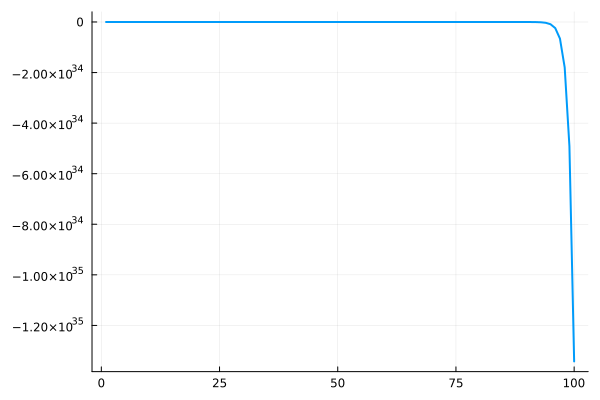
\includegraphics[scale=0.4]{plot32_1.png}
    \caption{Wyrazy ciągu obliczone przy użyciu wzoru rekurencyjnego w arytmetyce 32--bitowej.}
    \label{fig:plot32_1}
\end{figure}

\begin{figure}[!h]
    \centering
    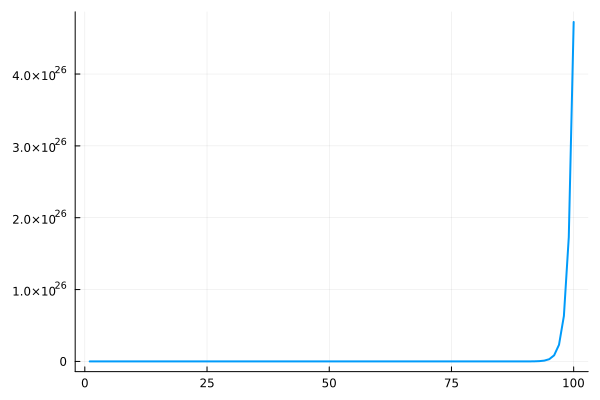
\includegraphics[scale=0.4]{plot64_1.png}
    \caption{Wyrazy ciągu obliczone przy użyciu wzoru rekurencyjnego w arytmetyce 64--bitowej.}
    \label{fig:plot64_1}
\end{figure}

Można zauważyć, że zaczynają się robić bardzo duże co do wartości bezwzględnej. Przyjrzyjmy się temu uważniej.

\newpage

%--------------------------------
% rekurencja -- 32 bity i 64 bity
%--------------------------------

\begin{table}[!h]
    \centering
    \begin{tabular}{|c|c|}
            \hline
             \(i\) & \(x_i\) \\
             \hline \hline
            10 &  -0.06044674 \\
            11 &  0.044008255 \\
            12 &  -0.03287697 \\
            13 &  0.022262573 \\
            14 &  -0.02122879 \\
            15 &  0.002067566 \\
            16 &  -0.03832245 \\
            17 &  -0.072509766 \\
            18 &  -0.22166443 \\
            19 &  -0.5883484 \\
            20 &  -1.6200256 \\
            \(\vdots\) &  \(\vdots\) \\
            96 &  \(-2.4096418 \cdot 10^{33}\) \\
            97 &  \(-6.5832636 \cdot 10^{33} \)\\
            98 &  \(-1.798581 \cdot 10^{34} \) \\
            99 &  \(-4.913815 \cdot 10^{34} \)\\
            100 &  \(-1.3424792 \cdot 10^{35} \) \\
            \hline
    \end{tabular}
    \caption{Obliczanie wyrazów ciągu przy użyciu arytmetyki 32--bitowej.}
    \label{tab:rek_32}
\end{table}

\begin{table}[!h]
    \centering
    \begin{tabular}{|c|c|}
            \hline
             \(i\) & \(x_i\) \\
             \hline \hline
            25 &  0.0005619005387416109 \\
            26 &  -0.00040833884304447565 \\
            27 &  0.0003071233913942706 \\
            28 &  -0.00020243090330041014 \\
            29 &   0.0002093849761877209 \\
            30 &  \(0.0000139081457746215\) \\
            31 &  0.0004465862439246848 \\
            32 &  0.0009209887793986127 \\
            33 &  0.002735150046646595 \\
            34 &  0.007312277652090415 \\
            35 &  0.02009485539747402 \\
            \(\vdots\) &  \(\vdots\) \\
            96 &  \(8.479372232653297 \cdot 10^{24}\) \\
            97 &  \(2.3166075755897554 \cdot 10^{25}\) \\
            98 &  \(6.3290895977101705 \cdot 10^{25}\) \\
            99 &  \(1.7291394346599854 \cdot 10^{26}\) \\
            100 &  \(4.724096788862005 \cdot 10^{26}\) \\
            \hline
    \end{tabular}
    \caption{Obliczanie wyrazów ciągu przy użyciu arytmetyki 64--bitowej.}
    \label{tab:rek_64}
\end{table}


%-----------------------------------------------
% rekurencja -- 32 bity i 64 bity - wykresy log.
%-----------------------------------------------

\newpage

\begin{figure}[!h]
    \centering
    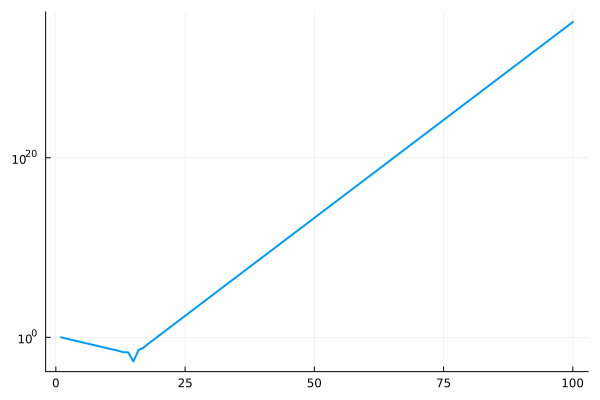
\includegraphics[scale=0.4]{plot32_log_1.png}
    \caption{Wykres funkcji \(f(n) = \ln(|x_n|)\), gdzie \(x_n\) obliczono przy użyciu wzoru rekurencyjnego w arytmetyce 32--bitowej.}
    \label{fig:plot32_log_1}
\end{figure}

\begin{figure}[!h]
    \centering
    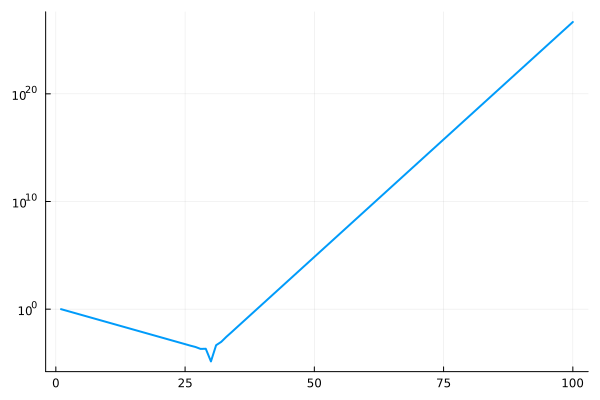
\includegraphics[scale=0.4]{plot64_log_1.png}
    \caption{Wykres funkcji \(f(n) = \ln(|x_n|)\), gdzie \(x_n\) obliczono przy użyciu wzoru rekurencyjnego w arytmetyce 64--bitowej.}
    \label{fig:plot64_log_1}
\end{figure}


Jak widać w tabeli w arytmetyce 32--bitowej wyrazy o indeksach 16 i 17 mają ten sam znak, natomiast w arytmetyce 64--bitowej dzieje się tak dla wyrazów o indeksach 29 i 30. Na wykresach \ref{fig:plot32_log_1} i \ref{fig:plot64_log_1} możmy zaobserwować, że rzeczywiście dla wyrazów o mniejszych indeksach obserwujemy, że maleją one z szybkością wykładniczą, natomiast od tego miejsca zaczynają wykładniczo rosnąć.  

Istotnie, łatwo zauważyć, że gdy \(x_i\) oraz \(x_{i+1}\) mają ten sam znak, to także \(x_{i+2}\) będzie tego samego znaku. Ponadto na mocy wzoru (\ref{wzor_rek}) otrzymamy, że 
\(\left| x_{i+2} \right| = 2\left| x_{i} + x_{i+1} \right| \geq 2 \left| x_{i+1} \right|\).

Ze wzoru (\ref{wzor_jaw}) można wywnioskować, że dla dowolnego \(i\) znak \(x_i\) powinien być różny od znaku \(x_{i+1}\). Stąd wnioskujemy, że jesteśmy świadkami poważnego błędu numerycznego, który sprawia, że ciąg \(x_k\) zamiast zbiegać do 0, zaczyna rozbiegać do \(\pm \infty\).

\newpage

\subsection{Sposób 2 -- wzór jawny}

W tej sekcji skorzystamy ze wzoru (\ref{wzor_jaw}) dla stałych \(A,B\) wyliczonych w Lemacie \ref{lem:stale}.

%------------------------------------------
% wzor jawny -- 32 bity i 64 bity - wykresy
%------------------------------------------

\begin{figure}[!h]
    \centering
    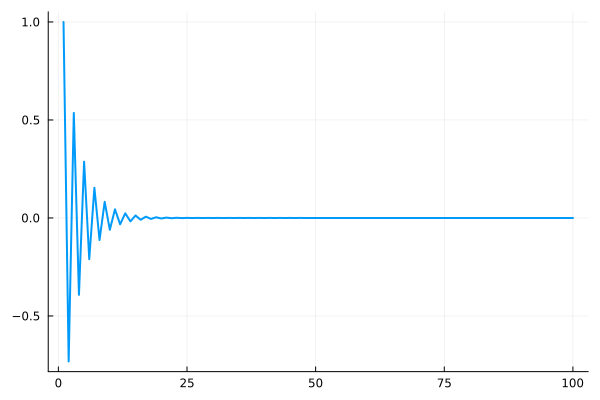
\includegraphics[scale=0.4]{plot32_2.png}
    \caption{Wyrazy ciągu obliczone przy użyciu wzoru jawnego w arytmetyce 32--bitowej.}
    \label{fig:plot32_2}
\end{figure}

\begin{figure}[!h]
    \centering
    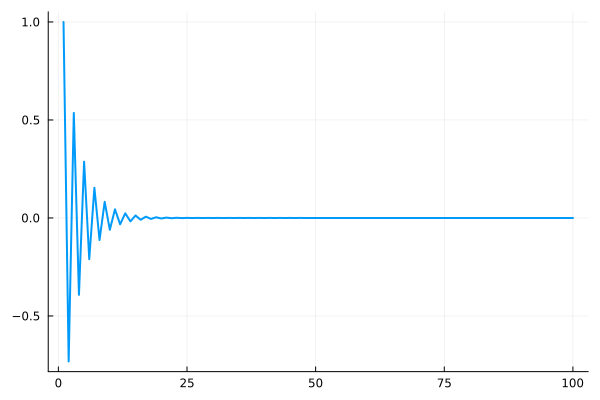
\includegraphics[scale=0.4]{plot64_2.png}
    \caption{Wyrazy ciągu obliczone przy użyciu wzoru jawnego w arytmetyce 64--bitowej.}
    \label{fig:plot64_2}
\end{figure}

Z wykresu odczytujemy, że tak obliczone wyrazy ciągu zbiegają do 0. Przyjrzyjmy się bliżej wynikom. 

%--------------------------------
% wzor jawny -- 32 bity i 64 bity
%--------------------------------

\newpage

\begin{table}[!h]
    \centering
     \begin{tabular}{|c|c|}
            \hline
             \(i\) & \(x_i\) \\
             \hline \hline
            90 &  \(-8.7936765 \cdot 10^{-13} \) \\
            91 &  \(6.437418 \cdot 10^{-13} \) \\
            92 &  \(-4.712517 \cdot 10^{-13} \) \\
            93 &  \(3.4498023 \cdot 10^{-13} \) \\
            94 &  \(-2.5254305 \cdot 10^{-13}\) \\
            95 &  \(1.8487436 \cdot 10^{-13} \) \\
            96 &  \(-1.3533743 \cdot 10^{-13} \) \\
            97 &  \(9.907387 \cdot 10^{-14}\) \\
            98 &  \(-7.2527115 \cdot 10^{-14} \) \\
            99 &  \(5.3093536 \cdot 10^{-14} \) \\
            100 &  \(-3.8867167 \cdot 10^{-14} \) \\
            \hline
    \end{tabular}
    \caption{Obliczanie wyrazów ciągu przy użyciu arytmetyki 32--bitowej}
    \label{tab:expl_32}
\end{table}

\begin{table}[!h]
    \centering
     \begin{tabular}{|c|c|}
            \hline
             \(i\) & \(x_i\) \\
             \hline\hline 
            90 &  \(-8.793645256554909 \cdot 10^{-13}\) \\
            91 &  \(6.437395111535248 \cdot 10^{-13} \) \\
            92 &  \(-4.712500290039321 \cdot 10^{-13} \) \\
            93 &  \(3.4497896429918525 \cdot 10^{-13}\) \\
            94 &  \(-2.525421294094934 \cdot 10^{-13} \) \\
            95 &  \(1.8487366977938358 \cdot 10^{-13} \) \\
            96 &  \(-1.3533691926021965 \cdot 10^{-13} \) \\
            97 &  \(9.907350103832773 \cdot 10^{-14} \) \\
            98 &  \(-7.252683644378381 \cdot 10^{-14} \) \\
            99 &  \(5.309332918908782 \cdot 10^{-14} \) \\
            100 &  \(-3.8867014509391976 \cdot 10^{-14} \) \\
            \hline
        \end{tabular}
    \caption{Obliczanie wyrazów ciągu przy użyciu arytmetyki 64--bitowej}
    \label{tab:expl_64}
\end{table}


%-----------------------------------------------
% wzor jawny -- 32 bity i 64 bity - wykresy log.
%-----------------------------------------------

\newpage

\begin{figure}[!h]
    \centering
    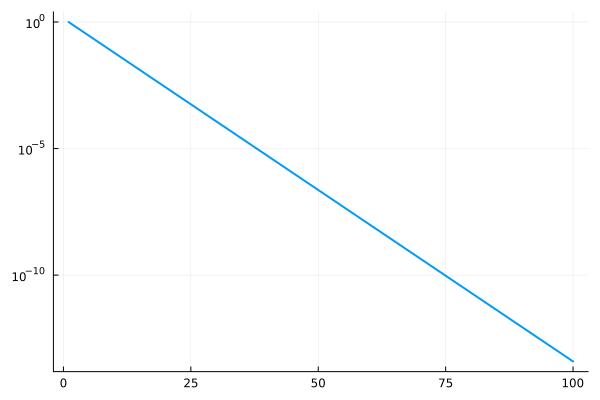
\includegraphics[scale=0.4]{plot32_log_2.png}
    \caption{Wykres funkcji \(f(n) = \ln(|x_n|)\), gdzie \(x_n\) obliczono przy użyciu wzoru jawnego w arytmetyce 32--bitowej.}
    \label{fig:plot32_log_2}
\end{figure}

\begin{figure}[!h]
    \centering
    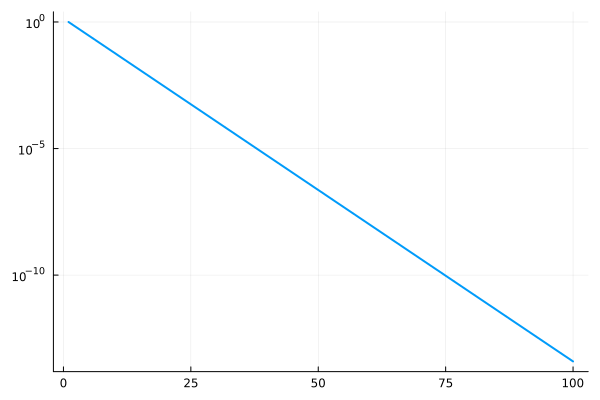
\includegraphics[scale=0.4]{plot64_log_2.png}
    \caption{Wykres funkcji \(f(n) = \ln(|x_n|)\), gdzie \(x_n\) obliczono przy użyciu wzoru jawnego w arytmetyce 32--bitowej.}
    \label{fig:plot64_log_2}
\end{figure}

Istotnie ten wzór podaje nam wyrazy ciągu z dobrym przybliżeniem. Widzimy, że ciąg maleje z szybkością wykładniczą, a jego zbieżność do 0 jest liniowa. Taki wynik mogliśmy przypuszczać, ponieważ nie wykonujemy tutaj żadnych ,,ryzykownych'' numerycznie operacji. 

\newpage

\subsection{Wyjaśnienie}

Należy zadać sobie pytanie, dlaczego w sposobie pierwszym błąd był aż tak drastyczny. Zauważmy, że gdy mamy \(x_2 = 1 - \sqrt{3}\), to w komputerze jest tak naprawdę \(x_2 = \text{fl}(1 - \sqrt{3}) \). Wobec tego wyrazy ciągu, które obliczamy korzystając z uprzednio wyliczonych wyrazów, są obarczone błędem numerycznym. Oszacujemy wielkość \(\tilde{A}\) we wzorze rekurencyjnym z błędem wynikającym z zaokrągleń w reprezentacji maszynowej, a w tym celu skorzystamy ze wzorów uzyskanych w dowodzie Lematu \ref{lem:stale}.

\begin{align*}
    \tilde{A} &= \frac{\text{fl}(x_1)(-2-2\sqrt{3}) - \text{fl}(x_2)(1-\sqrt{3})}{4\sqrt{3}}
    = \frac{-2-2\sqrt{3} - (1-\sqrt{3})(1 + \epsilon)(1-\sqrt{3})}{4\sqrt{3}} \\
    &= \frac{-2-2\sqrt{3} - (1-\sqrt{3})(1-\sqrt{3}) -\epsilon(-2-2\sqrt{3})}{4\sqrt{3}} \\
    &=  \frac{-\epsilon(-2-2\sqrt{3})}{4\sqrt{3}} =  \frac{\epsilon(1+\sqrt{3})}{2\sqrt{3}} \text{,}
\end{align*}

\noindent gdzie \(|\epsilon| \leq 2^{-t-1}\). Wobec tego 
\begin{align*}
    \left| \epsilon \right| > \left| \tilde{A} \right|  > \left| \frac{\epsilon}{2} \right| > 0 \text{,}
\end{align*}
ponieważ \(\epsilon \neq 0 \).

\noindent W szczególności \(\tilde{A} \neq 0\). Wobec tego zaobserwujmy, co się dzieje, gdy \(\tilde{A} \neq 0\). Przyjmijmy \(\tilde{A}\) bardzo małe co do wartości bezwzględnej, na przykład \(\tilde{A} = 2^{-t}\).

%--------------------------------------------
% wzor rek. II -- 32 bity i 64 bity - wykresy 
%--------------------------------------------

\begin{figure}[!h]
    \centering
    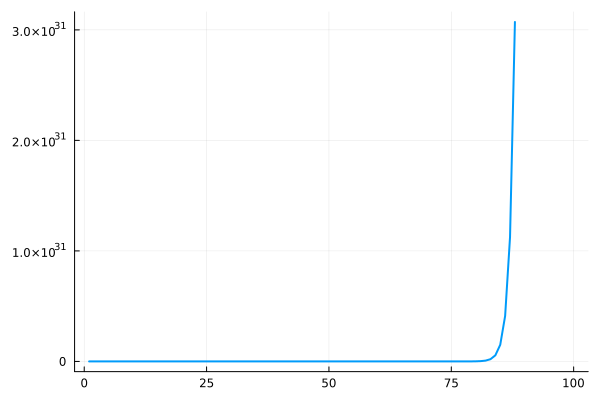
\includegraphics[scale=0.4]{plot32_3.png}
    \caption{Wyrazy ciągu obliczone przy użyciu wzoru jawnego dla \(\tilde{A} = 2^{-t}\) w arytmetyce 32--bitowej.}
    \label{fig:plot32_3}
\end{figure}

\newpage

\begin{figure}[!h]
    \centering
    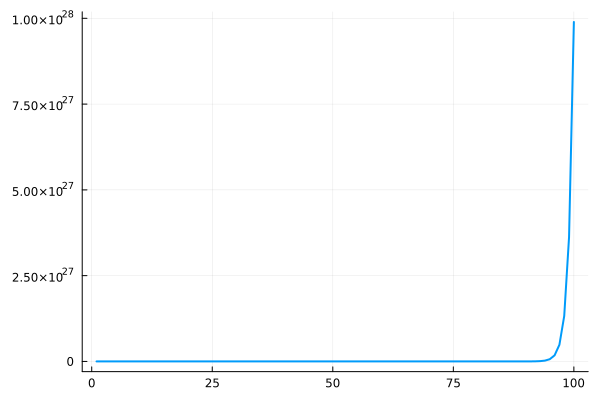
\includegraphics[scale=0.4]{plot64_3.png}
    \caption{Wyrazy ciągu obliczone przy użyciu wzoru jawnego dla \(\tilde{A} = 2^{-t}\) w arytmetyce 64--bitowej.}
    \label{fig:plot64_3}
\end{figure}

%--------------------------------------------------
% wzor rek. II  -- 32 bity i 64 bity - wykresy log.
%--------------------------------------------------

\begin{figure}[!h]
    \centering
    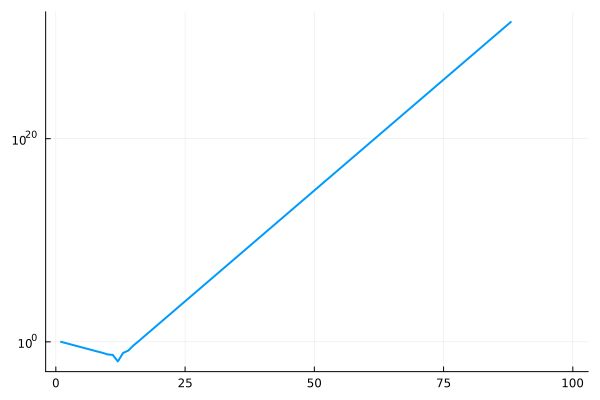
\includegraphics[scale=0.4]{plot32_log_3.png}
    \caption{Wykres funkcji \(f(n) = \ln(|x_n|)\), gdzie \(x_n\) obliczono przy użyciu wzoru jawnego w arytmetyce 32--bitowej dla \(\tilde{A} = 2^{-t}\).}
    \label{fig:plot32_log_3}
\end{figure}

\begin{figure}[!h]
    \centering
    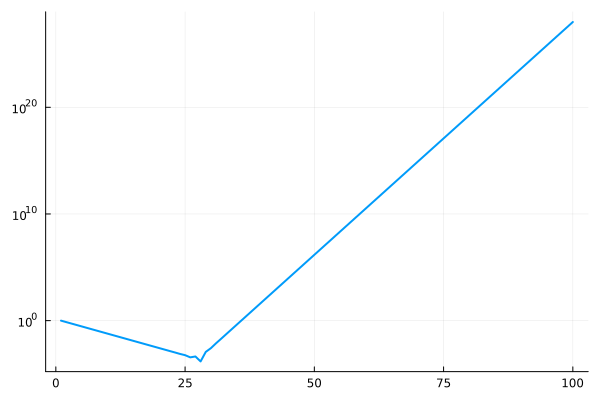
\includegraphics[scale=0.4]{plot64_log_3.png}
    \caption{Wykres funkcji \(f(n) = \ln(|x_n|)\), gdzie \(x_n\) obliczono przy użyciu wzoru jawnego w arytmetyce 64--bitowej dla \(\tilde{A} = 2^{-t}\).}
    \label{fig:plot64_log_3}
\end{figure}

\noindent Istotnie nawet dla bardzo małego \(\tilde{A} \neq 0\) widzimy, że ciąg rozbiega do \(\infty\) i to z szybkością wykładniczą, co ilustrują wykresy \ref{fig:plot32_log_3} i \ref{fig:plot64_log_3}. Możemy zauważyć, że są one zbliżone kształtem do wykresów \ref{fig:plot32_log_1} oraz \ref{fig:plot64_log_1}. Wobec tego błąd numeryczny powstały w Sposobie 1 wynikał z zaokrąglenia maszynowego \(x_2 = 1 - \sqrt{3} \). 


\newpage

\section{Podsumowanie}

Reasumując, wzór jawny i rekurencyny służący obliczaniu wyrazów ciągu \(x_n\) różnią się poprawnością numeryczną. Przy wzorze jawnym (\ref{wzor_jaw}) wykonujemy bezpieczne numerycznie operacje (wielokrotnie mnożymy). Nie powinno nas zatem dziwić, że uzyskujemy ciąg zbieżny do 0, czyli zgodny z oczekiwaniami.

\noindent Natomiast we wzorze rekurencyjnym (\ref{wzor_rek}) wyliczamy wyrazy ciągu również zadanego wzorem (\ref{wzor_jaw}), ale dla zmienionych stałych \(A, B\) -- a zmiana wynika z błędu powstałego przy zaokrągleniu. Wobec tego składnik \( (1+\sqrt{3})^k \) zaczyna rozbiegać do \(\infty\), dominując składnik \( (1-\sqrt{3})^k \), który zbiega do 0. 

\noindent Zdecydowanie lepszy, bardziej poprawny wynik uzyskujemy przy wykorzystaniu wzoru jawnego (\ref{wzor_jaw}) do wyliczenia wyrazów ciągu \( x_n \).

\end{document}
